% This file was created with tikzplotlib v0.10.1.post9.
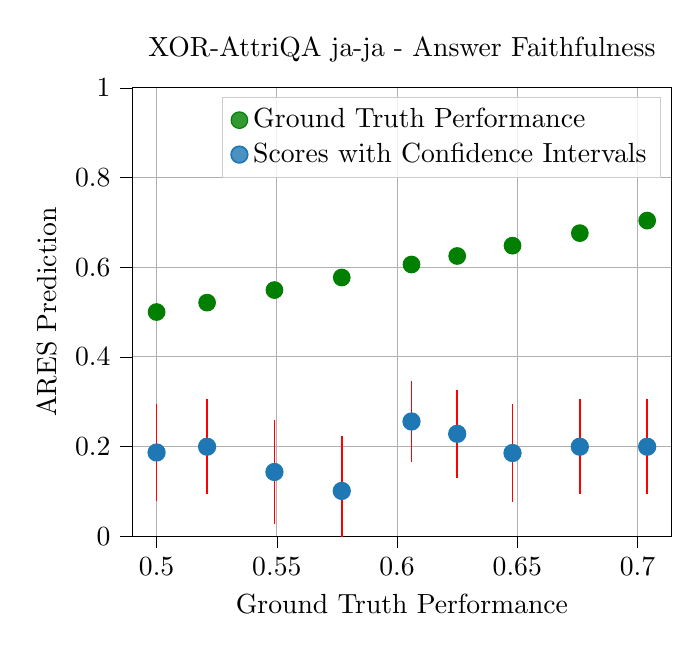
\begin{tikzpicture}

\definecolor{darkgrey176}{RGB}{176,176,176}
\definecolor{green01270}{RGB}{0,127,0}
\definecolor{lightgrey204}{RGB}{204,204,204}
\definecolor{steelblue31119180}{RGB}{31,119,180}

\begin{axis}[
legend cell align={left},
legend style={
  fill opacity=0.8,
  draw opacity=1,
  text opacity=1,
  draw=lightgrey204,
  mark options={mark size=3}
},
tick align=outside,
tick pos=left,
title={XOR-AttriQA ja-ja - Answer Faithfulness},
x grid style={darkgrey176},
xlabel={Ground Truth Performance},
xmajorgrids,
xmin=0.4898, xmax=0.7142,
xtick style={color=black},
y grid style={darkgrey176},
ylabel={ARES Prediction},
ymajorgrids,
ymin=0, ymax=1,
ytick style={color=black}
]
\addplot [draw=green01270, fill=green01270, mark size=3pt, mark=*, only marks]
table{%
x  y
0.5 0.5
0.521 0.521
0.549 0.549
0.577 0.577
0.606 0.606
0.625 0.625
0.648 0.648
0.676 0.676
0.704 0.704
};
\addlegendentry{Ground Truth Performance}
\path [draw=red, semithick]
(axis cs:0.5,0.079)
--(axis cs:0.5,0.295);

\path [draw=red, semithick]
(axis cs:0.521,0.094)
--(axis cs:0.521,0.305);

\path [draw=red, semithick]
(axis cs:0.549,0.027)
--(axis cs:0.549,0.26);

\path [draw=red, semithick]
(axis cs:0.577,-0.022)
--(axis cs:0.577,0.224);

\path [draw=red, semithick]
(axis cs:0.606,0.165)
--(axis cs:0.606,0.347);

\path [draw=red, semithick]
(axis cs:0.625,0.13)
--(axis cs:0.625,0.327);

\path [draw=red, semithick]
(axis cs:0.648,0.077)
--(axis cs:0.648,0.294);

\path [draw=red, semithick]
(axis cs:0.676,0.094)
--(axis cs:0.676,0.305);

\path [draw=red, semithick]
(axis cs:0.704,0.094)
--(axis cs:0.704,0.305);

\addplot [semithick, steelblue31119180, mark=*, mark size=3, mark options={solid}, only marks]
table {%
0.5 0.186666666666667
0.521 0.199577464788732
0.549 0.143239436619718
0.577 0.100985915492958
0.606 0.255915492957747
0.625 0.228333333333333
0.648 0.185492957746479
0.676 0.199577464788732
0.704 0.199577464788732
};
\addlegendentry{Scores with Confidence Intervals}
\end{axis}

\end{tikzpicture}
